\resetfigpath{Intro}


%%%%%%%%%%%%%%
%{Motivation}%
%%%%%%%%%%%%%%

The development of autonomous vehicles has grown rapidly as enabling technology emerges \cite{thrun2006}. Optimists claim that by 2030, most human drivers will be replaced by autonomous vehicles, while road congestion, accidents due to human errors, and air pollution problems can all be resolved\cite{JW2016}. To date, more than 47 autonomous vehicle companies are testing their self-driving cars in urban California \cite{CADMV} in 2019. However, practitioners believe that the penetration rate of fully-autonomous vehicles will remain low for the next decades. According to the work of Bansal et al. \cite{Prateek2017}, fully autonomous vehicles might take longer than expected to be ready in the market. Long-term (year 2015-2045) adoption rate of connected and autonomous vehicles (CAVs) under different scenarios is predicted to be 24.8\% at level 5 (as defined by the US Department of Transportation \cite{AV_levels2019}) by 2045. Regardless of the timeline of autonomous vehicles to be of great effects, evaluating the impact of autonomous vehicles needs to be done at a higher level, namely, how do people perceive and move around with autonomous vehicles, vehicles driven by  computers? 

%%%%%%%%%%%%%%%%%%%%%%%%
%% CONTENT : Problems %%

Impacts of autonomous vehicles have been assessed in various aspects of transportation. From the original intentions of reducing the number of accidents due to human errors, to alleviate traffic congestions\cite{Dresner2007, Ilgin2014}. However, if we consider the adaptation of autonomous vehicles from a city point of view, the impact might not all that positive. Studies argued that the reduction in the cost of traveling is likely to increase the total traveling distances for passengers which in turn exacerbate the congestion problem in urban areas\cite{EJTIR2017, MILLARDBALL2019} .

%%%%%%%%%%%%%%%%%%%%%%%%

In all scenarios, autonomous vehicles ultimately have to share the roads with human drivers. Apart from the fact that the technology itself is still at a preliminary stage where no commercially available level 4 vehicles exist in the market, neither are policy, infrastructure, and consumer acceptance ready for high adoption rate \cite{litman2015}. As a consequence, it is foreseeable that the \textit{mixed traffic flow} with both computer and human drivers will comprise the major part of the traffic during the transition stage that lasts for more than 30 years. Therefore, interactions between autonomous vehicles and the human environment will be the major challenge.

All new participants need to blend in the current traffic setup   smoothly. Urban traffic scenarios that include lane merging/diverging,  roundabouts, and crossroads without signals, rely heavily on driver interactions to predict and react accordingly. For example in Fig.\ref{INTERSECTION} we see an unsignalized crossroad for which drivers perceive and predict the possible intentions of others (shown as arrows in the figure), and then decide whether to accelerate or brake. These hints, as perceived by human drivers, are not understandable to autonomous vehicles nowadays, which might post a threat to surrounding drivers.

\begin{figure}[h!]
\begin{center}
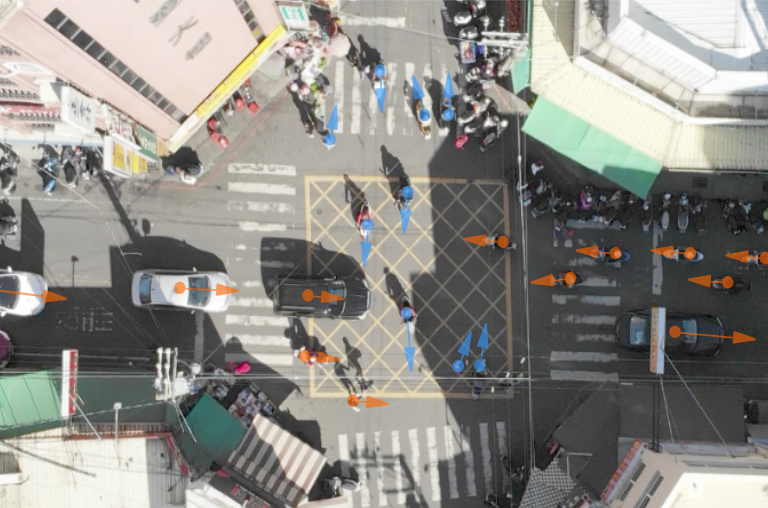
\includegraphics[scale=0.8]{complex_intersection_mod_demo.png}
\end{center}
\caption{A crossroad with no signal.}
\label{INTERSECTION} 
\end{figure}

The main reason for autonomous vehicles being potential threats to other road users is that they do not understand the meanings behind human behaviors and can not foresee their intentions. According to the report by the state of California Department of Motor Vehicles (DMV), 18 of the 33 filed accidents with autonomous vehicles in 2019 (as of June 17, 2019) are rear-ended\cite{CADMV}. Most accidents (over 60\%) happened as autonomous vehicles yielded unnecessarily for situations that following human drivers apparently did not anticipate. Autonomous vehicles are designed to drive conservatively for the cause of safety, but when those behaviours are not understandable to human drivers, over conservative autonomous vehicles become a new threat.

%%%%%%%%%%%%%%%%%%%%%%%%%%%%%%%%%%%%
%%  How interactions are studied  %%

To prevent the problem addressed, interactions with surrounding agents should be achieved by understanding their behaviors. Decisions based on purely control logics such as traditional collision avoidance systems suffer from insufficient reaction time as reported in \cite{Coelingh2010}. To warn drivers early enough to take proper actions, behavior prediction models are used, for example see  pedestrians predictions in \cite{Bonnin2014, Schneemann2016, HASHIMOTO2016}. In these studies, pedestrian crossing intentions are identified and modeled, making their behaviors comprehensible and thus greatly improve the safety of road users. Driver behaviors are also crucial for making safe decisions in traffic flow \cite{Ramyar2015, Gadepally2014}.
%%%%%%%%%%%%%%%%%%%%%%%%%%%%%%%%%%%%

Although modeling human intentions have been the focus of several existing studies, these models are however based on either extensive data collections that are difficult to adapt to new environments or implicit model framework that are intractable for on-line application. We study driver behaviors at unsignalized crossroads and build explicit probabilistic models in this work. Proper behavior model should enable computer drivers to understand and to interact with human drivers more smoothly, resulting in a safer human-computer mixed traffic flow. In what follows, we reviewed driver models in Section 2; our proposed probabilistic driver behavior models in unsigalized crossroads are presented in Section 3; Section 4 provides extensions of the driver model on some real world applications; Section 5 concludes the study with future work. 

% The primary goals as well as the process for the model construction are listed as follow:

% \begin{enumerate}

%     \item \textbf{Identification of driver decision making process} \\
%         How human drivers perceive and react to the traffic participants at the crossroad will be identified.
        
%     \item \textbf{Driver behaviors modeling}\\
%         Based on the current states of the target driver, a behavior model will be constructed based on the decision making process learned previously.
        
%     \item \textbf{Case study}\\
%         Possible applications using the proposed driver behavior model will be explored.

% \end{enumerate}


